\chapter{Amplifier \& Distortion}

\begin{center}
    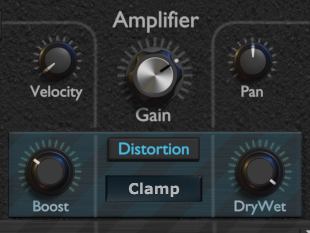
\includegraphics[width=0.4\textwidth]{graphics/amp_distortion.png}
\end{center}

The Amplifier and Distortion sections form the only parts in the signal flow in Odin 2 which are both polyphonic and stereo. 

\section{Amplifier}

The amplifier section plays an important gain-staging role in odin. The sound can be boosted or attenuated, as well as panned.

\audioparameter{Amp Gain}{1}{1}{
    Changes the volume in in deciBels. Can be used to shut the sound entirely. Modulating this parameter from the \modmatrix  with $-100$ will always shut the sound. Modulating this parameter with $+100$ will raise the sound to 0dB if the current value is smaller than -12dB. If it is bigger than -12dB, it will modulate to +12dB from the current value.
}

\audioparameter{Amp Pan}{1}{1}{
    Pan or Panorama can be used to move the sound over the stereo field. The default value of zero will leave the sound centered. Moving the pan towards -1 will attenuate the right stereo channel, moving towards 1 does the same for the left channel.

    \begin{center}
        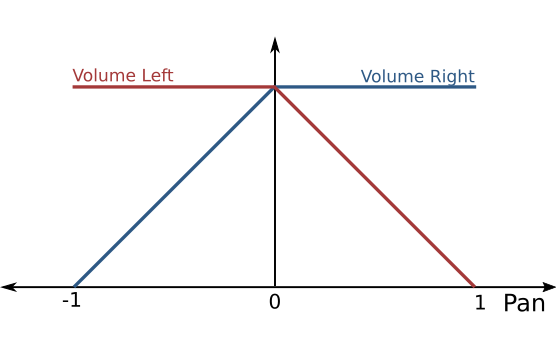
\includegraphics[width=0.7\textwidth]{graphics/pan_function.png}
    \end{center}
}

\audioparameter{Amp Velocity}{0}{1}{
    Makes the Amplifier gain sensible to the MIDI-Velocity. This allows for expressive play, where harder notes produce louder sounds. Increasing this value lowers the default gain of the amp, such that a MIDI-note with maximum velocity (127) will bring the level back to its previous level.
}

\begin{tcolorbox}[colback=yellow!10!white,
    colframe=white!20!black,
    center,
    valign=top,
    halign=left,
    center title,
    width=\textwidth]

Please note that the \hyperref[amp_env]{Amp Envelope} is not applied between the Amplifier and Distortion section, like the routing would suggest. The Amp Envelope is applied \fat{after the Distortion section}.
\end{tcolorbox}

\section{Distortion}

The Distortion module is capable of distorting the sound by various characteristic distortion functions. All the distortion types used in this section are threshold based: Once the wave surpasses a predefined value (in positive or negative direction), the processing will apply. Internally, 3x oversampling is used to prevent aliasing from the sharp cuts made to the waveform.

\audioparameter{Distortion On}{0}{1}{
    Turns the Distortion module on or off.
}

\vspace{20mm}
\audioparameter{Boost}{1}{1}{
    Boosts the incoming wave, to make it surpass the internal threshold easier.
}

\vspace{20mm}
\audioparameter{Dry Wet}{1}{1}{
    Interpolates the processed and unprocessed signals, thereby controlling the amount of distortion applied to the sound.
}

\vspace{20mm}
\audioparameter{Distortion Algorithm}{0}{0}{
    Selects which distortion algorithm is used. The options are:
    
    \vspace{7mm}
    \fat{Clamp}: 
    Clamps the signal once it surpasses the threshold.

    \begin{center}
        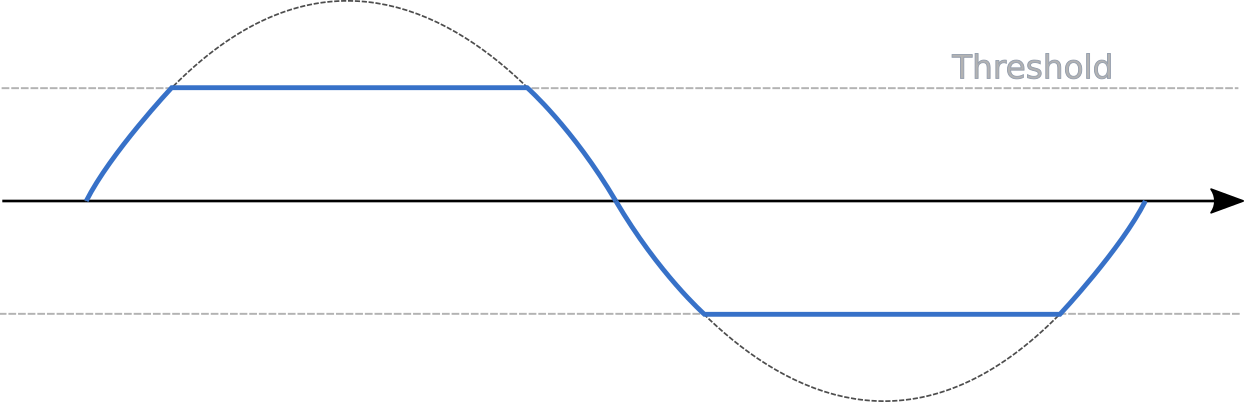
\includegraphics[width=0.7\textwidth]{graphics/overdrive.png}
    \end{center}

    \fat{Fold}: 
    Folds the wave over once it surpasses the threshold. If the folded wave hits the threshold on the other side, it will be folded again (and so on). Produces more harmonic content than the Clamp algorithm.

    \begin{center}
        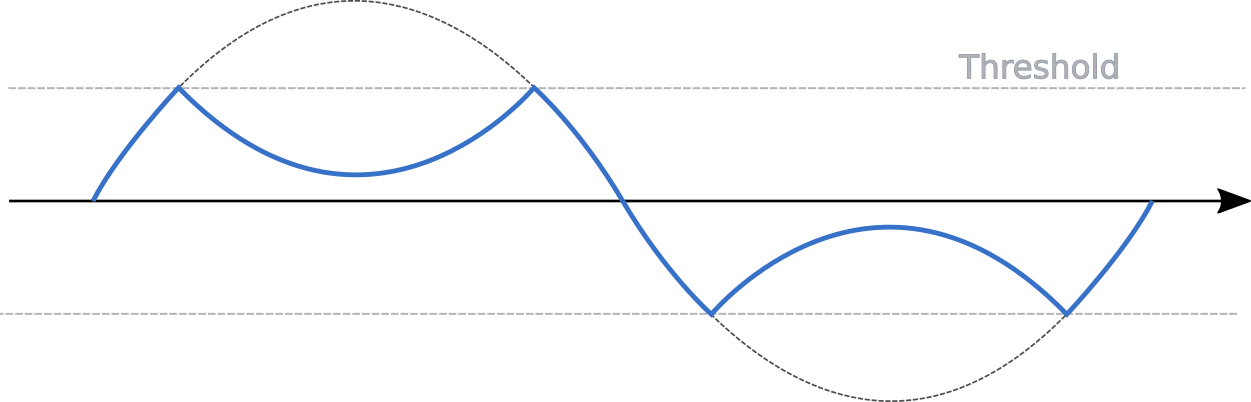
\includegraphics[width=0.7\textwidth]{graphics/fold.png}
    \end{center}

    \fat{Zero}: 
    Pulls the wave to zero once it surpasses the threshold. The strongest of the available distortion algorithms.

    \begin{center}
        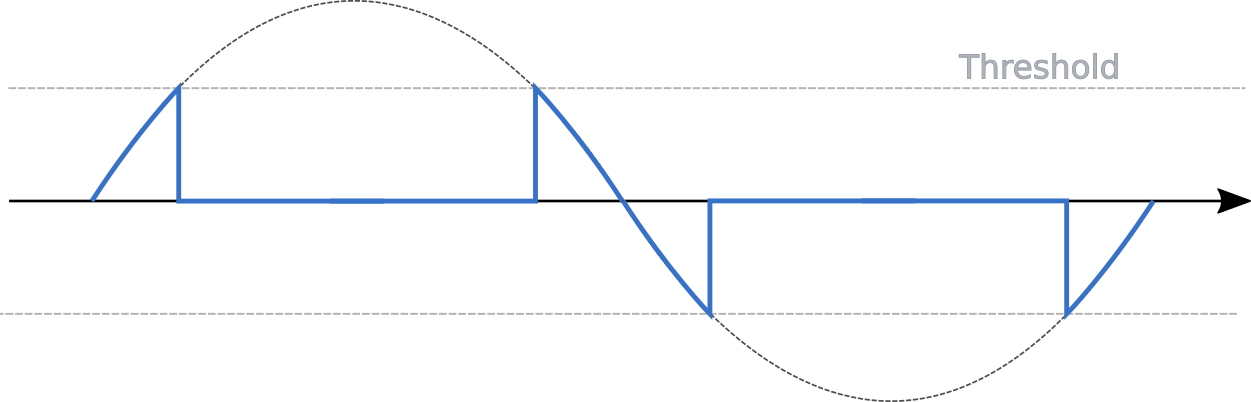
\includegraphics[width=0.7\textwidth]{graphics/zero.png}
    \end{center}
}
